\documentclass[12pt]{article}
\usepackage[ampersand]{easylist}
\usepackage{amsmath}
\usepackage{amsfonts}
\usepackage{amssymb}
\usepackage[obeyspaces]{url}
\usepackage{hyperref}
\usepackage{graphicx}
\usepackage[section]{placeins}


\title{Monitoring Memory and CPU Usage for Processes in Linux}
\author{Jatczak, David \and McNabb, Trent}

\begin{document}
	
	\maketitle
	
	\section{Introduction}
	
	\subsection{Context}
	Addressing this issue requires knowledge of what information is relevant to the calculation of memory and CPU (Central Processing Unit) resources, and how to get that information. Specifically, knowledge of the Linux \path{/proc/} files is needed.
	
	\subsection{Problem Statement}
	Computer users who are used to Windows might use \emph{Ctrl+Alt+Del} when they wish to see which processes are running and how much of the system's resources those processes are consuming. They may not be comfortable using the terminal to run commands that would display that information, or they might prefer to see the information in a GUI (Graphical User Interface) that looks more like the Windows Task Manager. A program that is accessible via the \emph{Ctrl+Alt+Del} keyboard shortcut that resembles the Windows Task Manager is needed. It should allow for a clear and easy view of which processes are running and what resources each process is using. It should be easy to terminate a running process.
	
	\subsection{Result}
We have created a program that binds automatically to the \emph{Ctrl+Alt+Del} keyboard shortcut. The program uses a GUI that is similar to the Windows Task Manager to display the list of all processes, the percentage of CPU resources and memory used by each process, the Process ID Number of each process, and the user name running each process. The program allows users to easily select and terminate processes. The program also displays the total memory usage and the total CPU usage. The program also shows which applications are running, and allows the user to select and end a task.
	
	\subsection{Outline}
	The rest of this report is structured as follows: Section 2 presents background information, including information about calculating system resource usage by specific processes using the Linux \path{/proc/} file; Section 3 describes in detail the program that we have written, which is the result of this project; Section 4 evaluates the result of the project, including with a usability study; Section 5 is the conclusion.
	
	\section{Background Information}
	The Linux \path{/proc} file system stores information about processes and also other system information.
Each process has a directory in the \path{/proc/} directory\cite[p. 792]{text}.
The directory is created at \path{/proc/[PID]/}, where PID (Process Identifier) is the process identification number. Each of these directories include a 'stat' file, a 'statm' file, and a 'status' file. In addition to the information about each process, there is also system information, i.e. the \path{/proc/cpuinfo} file and the \path{/proc/meminfo} file.\\
	The Resident Set Size in the number of pages that the process currently has in real memory.
	If we multiply that by the page size, which is a system variable, that gives the amount of RAM (Random-access Memory) currently used by the process.
	If we divide that by the total amount of memory used by the system, that will give us the percentage of system memory used by the process.
	The calculation is:\\
	$$ \frac{\text{Resident Set Size} \times \text{Page Size}}{\text{Total System Memory}} $$
	
	Information about the resident set size of a process can be found is \path{/proc/PID/statm} or\path{/proc/PID/stat} \cite{manProc}.
	Information about the total system memory and total free memory can be found in \path{/proc/meminfo} \cite{manProc}.\\
	To get the percentage of total memory in use by the system, the calculation is:\\
	$$ \frac{\text{Total System Memory} - \text{Free Memory}}{\text{Total System Memory}} \times 100 $$
	

A CPU can either be running or idle.
If it is running, it can be running a user space program, or running the kernel \cite{scoutBlog}.
If you add the time it is running the kernel, plus the time it is running a user space program, plus the amount of time it is idle, you get what we will call the Total CPU availability.
In order to do the calculation, we need to poll at a given interval and take the difference between the new data and the old data ($\Delta$) for those three variables. For example, if we say that the time running in user mode taken at $t_{1}$ is $U_{1}$, and the time running in user mode taken later at time $t_{2}$, then $$\Delta U = U_{2} - U_{1}$$. The calculation for total CPU availability is:\\
$$ \Delta\text{Running Userspace} + \Delta\text{Running Kernel Mode} + \Delta\text{Idle}$$
The calculation for the process CPU percentage is:\\
$$ \frac{\Delta\text{Process CPU user mode} + \Delta\text{Process Kernel mode}}{\text{Total CPU Availability}} \times 100 $$
The calculation for total CPU usage is\\
$$ \frac{\Delta\text{Running Userspace} + \Delta\text{Running Kernel Mode}}{\text{Total CPU Availability}} \times 100 $$
The amount of time that a process has been running in user mode and the amount of time that the process has been running in kernel mode can be found in \path{/proc/[PID]/stat}. \cite{manProc}
The total time spent by the CPU running user space processes, the amount of time running the kernel and the amount of CPU Idle can be found in \path{/proc/stat} \cite{manProc}.\\
	
	
Shortcuts, also known as hotkeys, that give functionality to applications are typically handled by an event handler.
Whenever a user presses a key on an operating system, an event is made and sent out for the event handlers to handle.
There are many more types of events than key presses and key releases, such as mouse movements, and GUI events.
Event handlers are in event loops. Event loops are embedded in applications themselves and/or in the operating system. Simple processes such as shell tools do not typically have event handlers, but many modern applications do. The typical structure of an event loop is that goes through the queue of events it has, does what it needs and then chooses to dispatch the event or not, afterwards waiting for more events. 

The Qt framework offers a library that gives GUI functionality and is based in C++, but it also used in other languages such as Python where it has been ported.
The Qt framework has an event loop and receives its events from windowing systems such as X11 or Wayland.
If you are interested in this topic, it is explained further by Thiago Macieira in his powerpoint on the Qt event loop\cite{QtSlides}.

For this text, we use X11 as our window system.
X11 is the base of the GUI system for Linux.
It handles all the communication between the user input and other windows because it is the framework that other applications are working off.
X11 has its own event loop, and is basically at the top of the hierarchy of event loops.

To interact with X11's event loop, you require a library such as Xlib or XCB.
XLib was made by the same company that created X11.
XCB is a faster alternative to Xlib and is asynchronous.
Both of these libraries communicate with X11 via binary because X11 uses a client-server design for its system.

Unity is the desktop environment for Ubuntu, it operates with X11 (by default). Unity is able to use .desktop files to launch applications.
These .desktop files are in plaintext and assign key-value pairs such as what command to execute.
An option to launch the files upon startup is done by putting them in \path{~/.config/autostart}.
Unity also has custom shortcuts available that can execute commands.
The configuration of shortcuts are separate for each each user and are located in the user's \path{~/.config/dconf}.
The configuration files are not plaintext, so the only way to change the configurations by terminal is through the command \path{gsettings}.


	
\section{Result}

The GUI layout was created in Qt Designer, which outputs a '.ui' file, which is an file in XML (Extensible Markup Language).
That '.ui' file is compiled by a PyQt5 utility called pyuic5 that generates the file that run the GUI. In our program, this file is 'UImainwindow.py'. Our program  'overseer.py', imports this file, as well as the PyQt5 libraries. 
'Uimainwindow.py' has a class called Ui\_MainWindow that allows the creation of Ui\_MainWindow objects.
If changes are needed to the GUI, the changes need to be made to the '.ui' file, and the 'Uimainwindow.py' file needs to be generated again.
When the main function is run in 'overseer.py', it creates an Ui\_MainWindow object, runs the OverseerMainWindow function and tells the Ui\_MainWindow object to show on the screen.\\
The OverseerMainWindow function creates the the model for the table that holds the data so that the UI can display it.
It creates an instance of the Proc class from 'proc.py'.
The OverseerMainWindow function calls the update function, which updates the data by calling the readData function on the Proc object and then updates the view by calling the updateView function.
It repeats this once every second.\\
The Proc object stores the following data: a dictionary called processList, a UserList object called userList, from 'userlist.py', an integer called totalMem, two strings called memStr and cpuStr, and two lists called cpu and openWindows.\\
The readData function runs the functions that populate each of those data members.
readTotalMem gets the total memory usage and free memory from \path{/proc/meminfo}. It stores the total memory in totalMem and uses the total memory and the free memory to calculate the total memory percentage. It converts it to a string and stores it in memStr.\\
See Figure ~\ref{figTotalMem}.
The circled data is the data stored as totalMem and the freeMem in the Proc object.\\
\begin{figure}[h]
	\centering
	\textbf{Total Memory}\par\medskip
	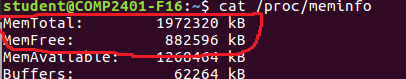
\includegraphics{totalMem}
	\caption{Output of \url{cat /proc/meminfo}}
	\label{figTotalMem}
\end{figure}
The readcpuTimes function gets CPU information from \path{/proc/stat} and creates a CPU object using the cpu.py file. the CPU object stores the amount of time the CPU has been running user space programs as usertime, the ammount of time the CPU has been running kernel mode as systime, and the amount of idle time as idletime.
It also has a variable called period, to store the total CPU availability, as discussed in the background.\\
See Figure ~\ref{figCPUInfo}.
The circled data are the numbers put in the list cpu.
This is the combined data for all processors in the system.
The first number is the time spent in user mode.
The third number is the time spent in system mode.
The fourth number is the time spent in idle.
None of the other numbers are relevant for our purposes.\\
\begin{figure}[h]
	\centering
	\textbf{CPU Information}\par\medskip
	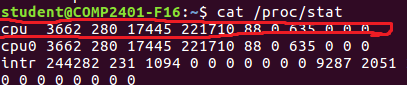
\includegraphics{totalCPU}
	\caption{Output of \url{cat /proc/stat}}
	\label{figCPUInfo}
\end{figure}
The readProcListData function gets the list of processes using the os library from python. It walks the list, and for every PID, it creates a Process object that stores 12 variables. The are 10 strings, called name, fullname, fullpath, path, rss, utime, stime, state, fullState and windowName. There are 4 numbers, called pid, realUid, ramPercentage and cpuPercentage. The readProcList function walks the list of processes, it gets information from \path{/proc/status} to populate the realUid field (See Figure ~\ref{figRealUid}, where the real user ID is circled in red), and \path{/proc/stat} to populate name, state, rss, utime, and stime. name is the process name. rss is the Resident Set Size, meaning how many pages the process has in memory. utime is the amount of time the process has been scheduled to the CPU in user mode. stime is the amount of time that the process has been scheduled to the CPU in kernel mode. See Figure ~\ref{figProcPidStat}. The data for the following fields are circled in red: name and state, rss and utime and stime It checks processList, which is the process list from the last poll in order to get the process previous utime and previous stime. It uses the new data and the old data to calculate the difference. It uses that information to calculate the process CPU percentage, which it stores in cpuPercentage. 
It uses RSS (Resident Set Size) and totalMem to calculate the process memory usage.
It then tries to populate fullpath out of \path{/proc/PID/exe}, which contains the actual path name of the executed command \cite{manProc}. It is a symbolic link and needs to be deferenced. It then adds the Process object containing the data to a temporary variable. Once it has finished enumerating the entire list of processes, it makes the temporary variable containing all the data from this run through into the new processList variable, so that it has the data that it needs the next time it is run.\\
The readOpenWindow uses a 3rd party command line tool called wmctrl\cite{wmtrl} to get the open windows, and then filters them so it doesn't show the Ubuntu windows driving the desktop.
\begin{figure}[h]
	\centering
	\textbf{Real User ID}\par\medskip
	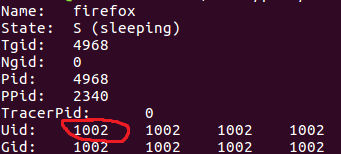
\includegraphics{realUid}
	\caption{Output of 'cat /proc/status'}
	\label{figRealUid}
\end{figure}
\begin{figure}[h]
	\textbf{Data for Process Object}\par\medskip
	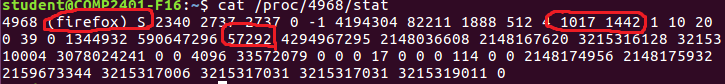
\includegraphics{procPidStat}
	\caption{Output of 'cat /proc/PID/stat'}
	\label{figProcPidStat}
\end{figure}
\\To show that the program is getting accurate numbers for CPU and Memory usage, I have included Figure ~\ref{figCompare}.
\begin{figure}[h]
	\centering
	\textbf{Comparison to Top}\par\medskip
	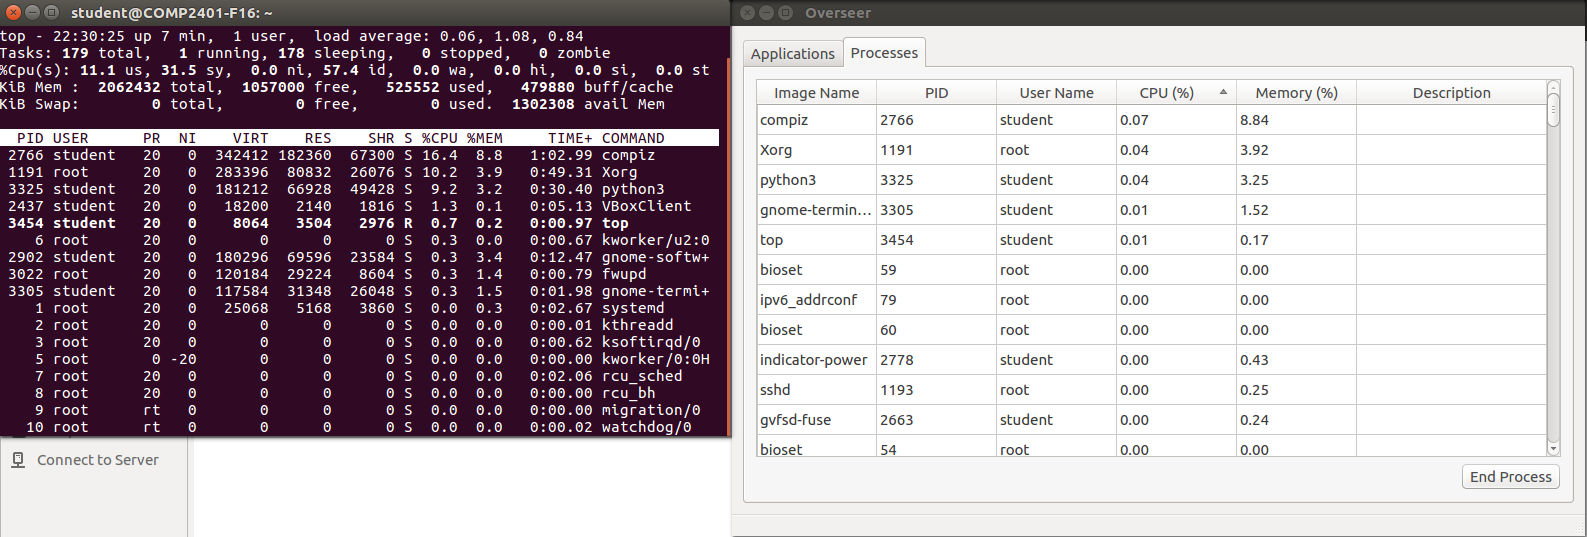
\includegraphics{compareToTop}
	\caption{Comparison to Output of Top}
	\label{figCompare}
\end{figure}

Overseer is able to calculate its CPU usage and RAM usage through polling.
The interval for polling is every second.
The data that is used for polling is describing running processes and the operating system and is stored on \path{/proc}.
Reading these files may seem like a strain, but there should not be any overhead from IO blocking since these files in \path{/proc} are virtual files and not actual files on a disk.
Virtual files are stored only on RAM (Random-access Memory), also known as the main memory.
In theory you should be able to read all the info from \path{/proc} almost instantly.
Thus having 1 second of polling should not be too bad for a single threaded program.

When all this data is collected from \path{/proc}, we also perform our CPU and RAM usage calculations as well as collecting a list of users.
The list of users is collected at the start of the poll cycle.
Collecting a list of users gives overhead as there is possible IO blocking from reading \path{/etc/passwd} because this is not a virtual file but an actual file on the disk.
Information on open windows in the window manager is collected through \path{wmctrl} and might give overhead as well depending on how wmctrl operates; window information is also collected in each poll cycle. 

The original goal was to have Overseer launch upon startup and it would sit in the system tray, where it would show the window when the shortcuts \emph{Ctrl+Alt+Del} or \emph{Ctrl+Shift+Escape} was pressed.
Overseer would have used an event handler for detecting the shortcuts (key press events).
If a key release event was detected for either key in a shortcut before all 3 keys having a key press event, the check for the shortcut would fail.
Implementation for putting a .desktop file in \path{~/.conf/autostart} did manage to get the program to launch on startup. But if the user were to log out and log back in, it would not launch again.

However, the main crux is the issue of reading events from X11 within the main thread of the application, which Qt operated off.
The Qt framework only provided ways to have working shortcuts if the Qt application itself is in focus, meaning it is unable to read key presses when the Qt application is minimized or selected to receive user input.
So another library was needed to read key press events, which led to Xlib.

Utilizing Xlib to read key presses with Python 3.5.2 is possible.
There is an example at \path{/usr/share/doc/python3-xlib/examples/record_demo.py} that illustrates reading events.
However, due to our lack of knowledge with Xlib and the poor documentation \cite{badDocumentation} for the Python version of Xlib, the event loop could not be changed to our liking.

Essentially the call back loop handles all the events coming from X11, then keeps calling itself to handle more events.
This call back loop was not possible to implement in our application's main thread because Qt operates off the main thread.
For example if \emph{time.sleep(5)} were to be executed in the main thread, the GUI would stop working all together and look frozen for 5 seconds.
This call back loop was the only thing executing so Qt did not operate.

It was thought it would be possible to implement the Xlib call back loop in another thread, a QThread, where this 2nd thread would check for key press events with its callback loop while the main Qt GUI thread would run.
However, it is incredibly dangerous when Xlib is used out of the main thread, as was explained to us by the Qt Core Maintainer Thiago Macieira over IRC.
Also to add, multithreading is not a wise idea with Qt in general.
The reason is you could have more overhead to Qt's main event loop if your threads were sending more events to the main thread's event loop. This is explained further by Qt's web page\cite{QtThreading}.

Thus XCB was turned to instead, as another way to read events.
A derived class of QAbstractNativeEventFilter, a class in the Qt framework, was created to handle the events coming from X11.
The type \url{xcb_generic_event_t} is sent to \url{QAbstractNativeEventFilter} by Qt.
Unfortunately, Python 3.5.2 does not recognize that type of data, and the PyQt5 library does not have an implementation of this data type either.
An XCB library was needed to understand the \url{xcb_generic_event_t} data.

Due to our entire application being programmed in Python 3.5.2, there are no decent libraries of XBC available.
Most libraries for XBC on Python are in the 2.x version of Python, e.g. \url{https://xcb.freedesktop.org/XcbPythonBinding/}.
Search engine results led to other XBC implementations in Pythyon 3.x such as \url{https://github.com/samurai-x/samurai-x/tree/master/pyxcb/pyxcb} or \url{https://github.com/tych0/xcffib}.
Both were unsuccessful for deciphering key press events from \url{xcb_generic_event_t} data.
There was some progress in deciphering the data, but there are many missing functions and constant values such as \url{XBC_MOUSE_PRESS}. The work can be seen from \url{http://github.com/Davidj361/Comp3000Group5/tree/global-shortcuts} and \url{http://github.com/Davidj361/Comp3000Group5/tree/global-shortcuts-method2}

Finally shortcut functionality was achieved with Unity's custom shortcuts.
Our Overseer does not deal with any events in the code, it merely interacts with Unity's custom shortcuts system.
Our application does not launch no longer on startup with a .desktop file, but instead launches from a bash file when a shortcut is pressed which in turn opens our Overseer application.
\emph{Ctrl+Alt+Del} or \emph{Ctrl+Shift+Escape}
Unfortunately the \emph{Ctrl+Shift+Escape} does not work.
The reason is because Ubuntu's shortcut manager does not work with \emph{Escape} as part of a shortcut, as illustrated in this bug report \url{https://bugs.launchpad.net/ubuntu/+source/compiz/+bug/158855}.

The applications tab in Overseer utilizes \path{wmctrl}\cite{wmtrl}, a 3rd party tool, to interact with windows in the desktop environment.
It collects information on windows showing in desktop environment and also gives the functionality for switching to a window.
Unfortunately \path{wmctrl} also collects information on junk windows such as 'Hud', 'unity-dash', 'unity-panel', 'unity-launcher', and 'XdndCollectionWindowImp', even if it's not on the desktop environment's taskbar.

Selections on the \emph{QtTableView}s in the process tab and applications tab has issues because Python does not have pointers.
It is hard to utilize Model View Controller design, which is the basis of \emph{QtTableView}, because we cannot link our data straight from Overseer's Proc class as a model to a QtTableView.
Instead, there's a poll cycle and new data is grabbed, all of the entries in each \emph{QtTableView} is erased and reinserted.
However, this gets rid of our selection every poll cycle. 
So Overseer remembers a \emph{PID} if there was a selection before the erase and reselects by iterating over the entire list in the \emph{QtTableView} looking for a matching PID, otherwise leaves no selection if not found.
Sadly this adds overhead to the main thread.	

	\section{Evaluation}
	We created a program that shows total CPU usage, total memory usage, a list of all processes and individual process information, such as memory usage, cpu usage, PID and user ID. We did a usability study, asking the 5 questions, all on a scale of 1 (Very Hard) to 5 (Very Easy). The questions were how easy is it to launch the program, find out what process are running, see process memory usage, see process CPU usage, and kill a program. We found that on average, people gave the program a rating of 4.95, with a standard deviation of .23. See Figure ~\ref{figUsage}. Unfortunately, there are other programs that do this that are also easy to use, such as the Ubuntu system monitor. People who are more familiar with widows might appreciate that our program looks very similar to the old Windows Task Manager, and that it automatically binds to the \emph{Ctrl + Alt + Del} shortcut. However, the Ubuntu System Manager is also very usable, and a user could choose to bind it to the \emph{Ctrl + Alt + Del}. We did not make a program that is superior to the Ubuntu System Manager.
	\begin{figure}[h!]
		\centering
		\textbf{Usability Study}\par\medskip
		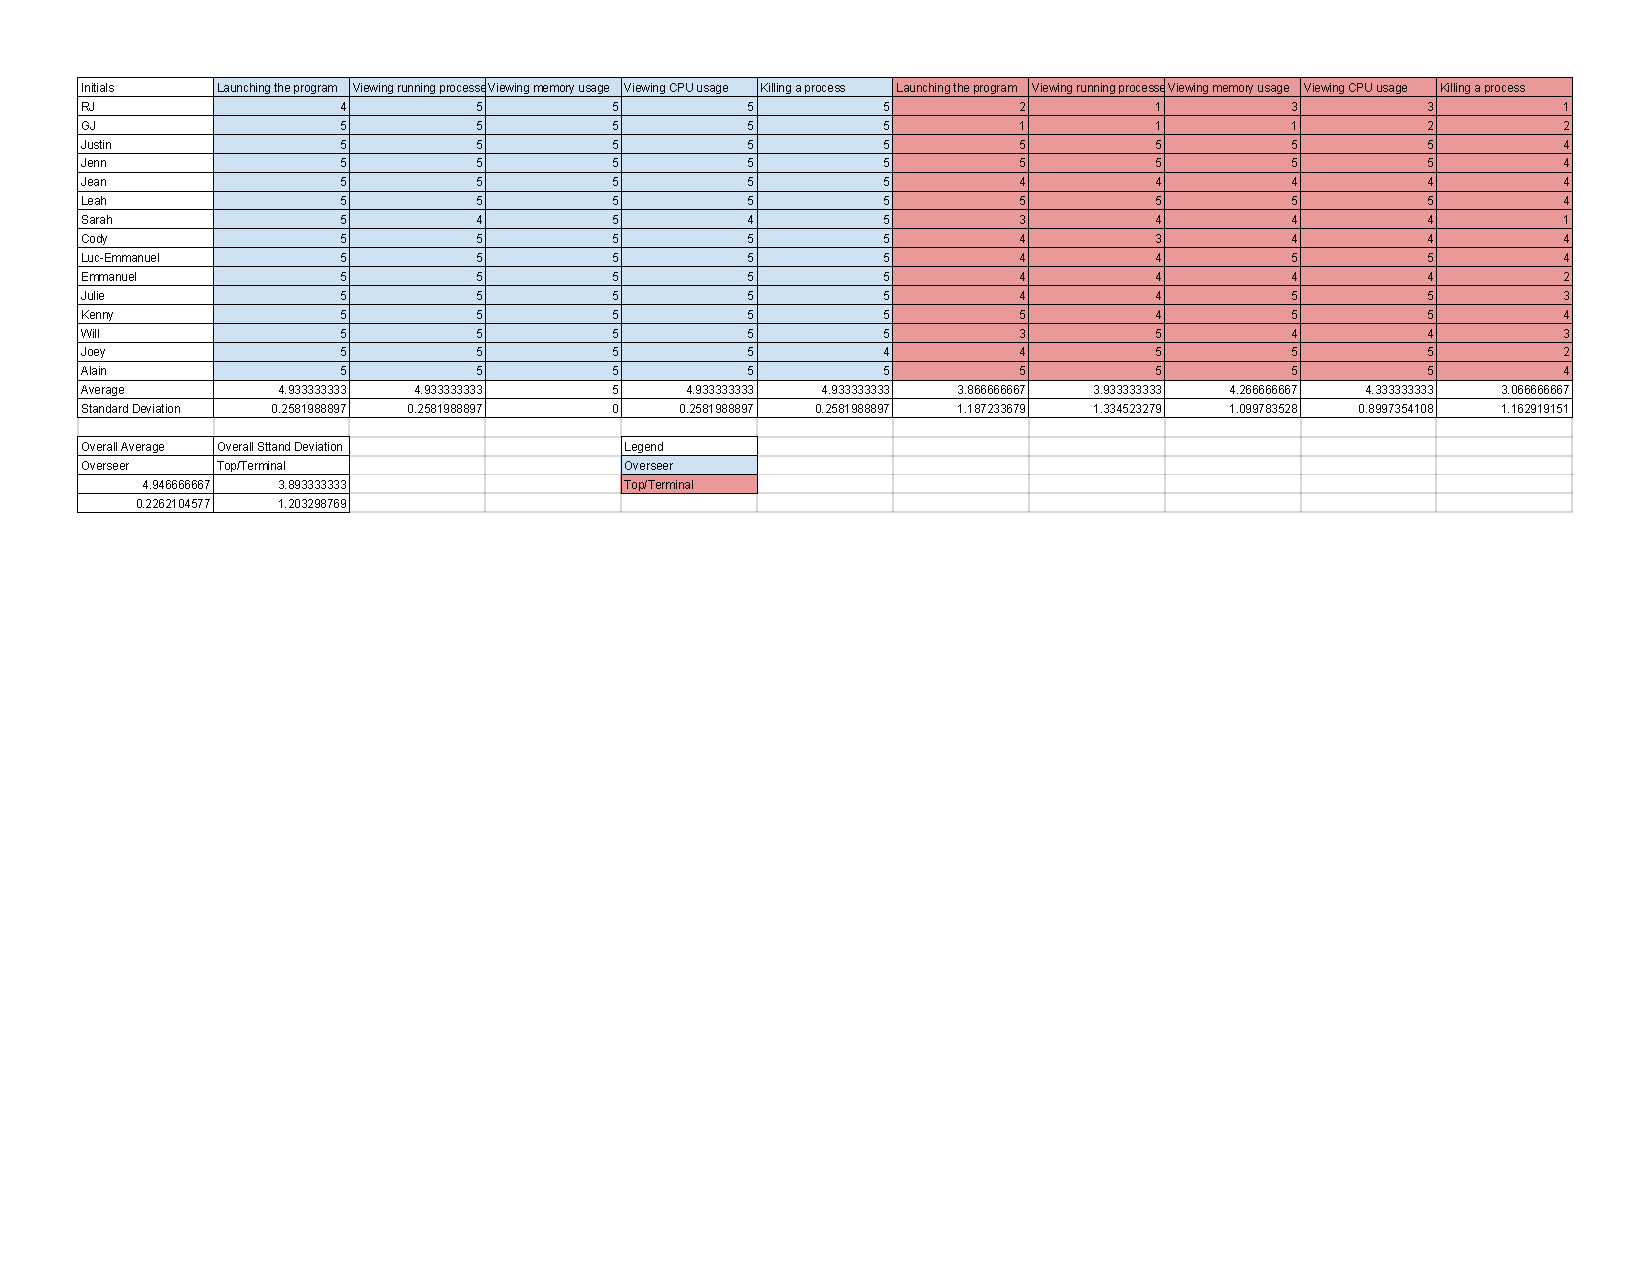
\includegraphics[scale=.7]{usageStudy}
		\caption{Data from Usability Study}
		\label{figUsage}
	\end{figure}
	
	\section{Conclusion}
	
	\subsection{Summary}
	We created a program that gets information from \path{/proc/meminfo}, \path{/proc/stat}, \path{/proc/PID/status}, \path{/proc/stat} and uses that information to calculate the total CPU usage, the total memory usage, each individual process CPU usage, each individual process memory usage. the program also gets the process user name, and allows users to end processes. It also displays a list of running applications, and allows users to end tasks. The program resembles the windows task manager, and it automatically binds to the \emph{Ctrl-Alt-Del} keyboard shorcut. The program refreshes the data once every second.
	
	\subsection{Relevance}
	Memory, the \path{/proc/} file, processes, process IDs and system calls were all covered in the course and used to varying degrees in the making of this project.
	
	\subsection{Future Work}
	There is significant further work that could be done on this project.
The program currently fails to end processes that aren't owned by the user running the program, but the process would have to run in kernel mode to do that.
The description field on the process tab is currently blank. The sort is currently a string sort, that doesn't quite get the order right. While that isn't an issue for sorting by the username, or by the process name, it is a problem for numerical fields like the PID. For example, it would order 1, 2, 11 as 1,11,2. In addition, the program might be able to differentiate itself if could show graphs, or output charts. 
	
	
	\setcounter{secnumdepth}{0}
	\section{Contributions of Team Members}

\ListProperties(Hide=100, Hang=true, Progressive=3ex, Style*=-- ,
Style2*=$\bullet$ ,Style3*=$\circ$ ,Style4*=\tiny$\blacksquare$ )

\subsection{Trent McNabb}
\begin{easylist}
	& For the Proc class:
	&& altered readTotalMem to get free memory.
	&& altered readcpuTimes to get the total CPU percentage.
	&& altered readcpuTimes to get the process information to return the correct information.
	& For the Overseer class:
	&& Implemented readTotals to output total CPU percentage and Memory Percentage to the status bar 
	& Original implementation of memory process percentage.
	&& David turned this implementation into a much cleaner implementation, with proper object oriented design, in the classes in the final product.
	& Implemented a method of killing process.
	&& David's implementation was used in the final program, is it was the better implementation.
	& Got the program to display the userID of each process.
	&& David completed this implementation by matching the userIDs to the username and displaying that information.
	& Designed the usability study.
	& For the Project Report Document:
	&& Sections 1, 4 and 5.
	&& For background section:
	&&& Information about the relevant CPU and memory calculations, and where to get the info from \path{/proc/}
	&& For the Results section:
	&&& Described the program logic, where the program gets the information to do the calculations, and how it does the calculations.
	
\end{easylist}		
	
\subsection{David Jatczak}
\begin{easylist}
& All of following classes: Process, CPU , UserList, and UserEntry
& For Proc class:
&& Implemented readcpuTimes, readOpenWindow; obtaining: process times, process CPU usage percentage, process paths, their permissions, process state.
& For OverseerMainWindow class:
&& Implemented Right-click context menus, selection logic for QTableViews, button logic, setupgsettings, setupLaunchScript, and setupShortcuts
& For the Project Report Document:
&& For the Background Section:
&&& Explaining Shortcuts, Events\&Event-Handlers\&Event-loops, X11, Unity, .desktop files
&& For the Results Section:
&&& Describing polling, overhead in polling, the failures of utilizing event handling, Unity's shortcut functionality, wmctrl, difficulty with MVC in QTableView, selection logic in QTableView
&& Proof read Trent's text
& Placement of GUI elements
& Reading htop's and top's source code to find RAM \& CPU usage calculations
& Research in event handling
\end{easylist}

\hfill\break
For more detail on contributions: \url{http://github.com/Davidj361/Comp3000Group5}
	
	
	
	\begin{thebibliography}{3}
	\bibitem{QtSlides} Thiago Macieira - Qt Core Maintainer \url{http://github.com/boostcon/cppnow_presentations_2013/blob/master/mon/qt_event_loop.pdf?raw=true}
	\bibitem{manProc} Proc(5) - Linux Manual Page
	\url{http://man7.org/linux/man-pages/man5/proc.5.html}
	\bibitem{text}{Tanenbaum, A. S. (2015). \emph{Modern operating systems.}}
	\bibitem{scoutBlog} Understanding Linux CPU stats \url{http://blog.scoutapp.com/articles/2015/02/24/understanding-linuxs-cpu-stats}
	\bibitem{badDocumentation} \url{/usr/share/doc/python3-xlib/html} \& \url{http://python-xlib.sourceforge.net/doc/html/index.html}
	\bibitem{QtThreading} \url{https://wiki.qt.io/Threads_Events_QObjects}
	\bibitem{wmtrl}Styblo, Tomas. \emph{WMCTRL}. Documentation at \url{http://tripie.sweb.cz/utils/wmctrl/}. Available under the GNU GPL.
	\end{thebibliography}


\end{document}
